\documentclass[Main]{subfiles}

\begin{document}


\section{Designprocess}

\subsection{Fjernbetjening}

Projektet skulle indeholde en sender som kunne sende kommandoer til dronen.

\begin{figure}[H]
\centering
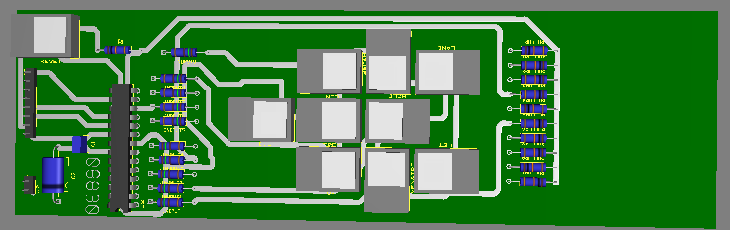
\includegraphics[width = 1 \textwidth]{3dUdenTal}
\caption{3D Figur af sender}
\label{Fig:3dUdenTal}
\end{figure}


Senderen som ses på figur \ref{Fig:3dUdenTal}, er bygget op i form som en fjernbetjening for, at det er muligt at betjene den med én hånd.
Fjernbetjeningen indeholder en µ-controller, radiosender og knapper.
Knapperne er her brugeren vælger et program/kommando der skal sendes til dronen. Når en knap bliver trykket ned, registrere µ-kontrolleren det. Denne genere så en frame med brugervalget. Denne frame bliver så sendt til radioen via SPI, hvorefter radioen får besked om at sende framen fra µ-kontrolleren.

\subsection{4+1 View}


\subsubsection*{Logic View}

Fjernbetjeningen udgør den største del af Use Casene beskrevet i kravspecifikationen\cite[s. 7 -- 11]{Kravspec}.

Et lille scenarie kunne optegnes og der kunne sættes nogle klasse navne på for, hvad der skulle være i de forskellige hardware-komponenter.

\begin{figure}[H]
\centering
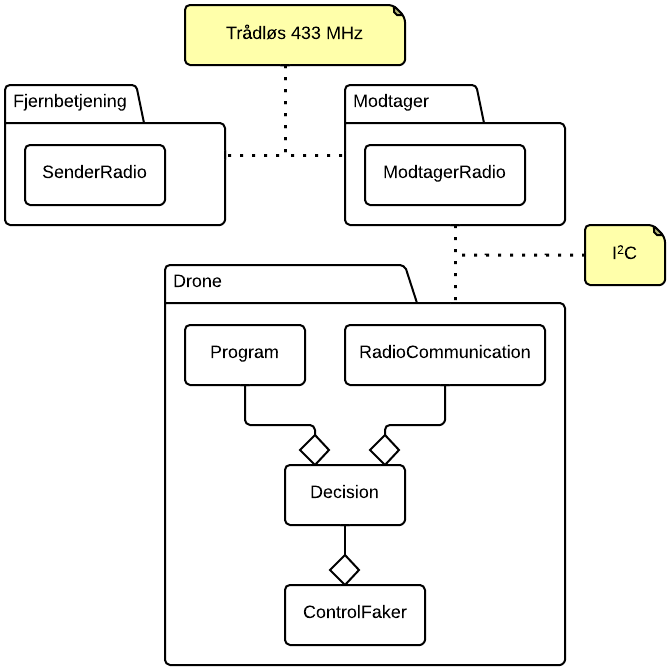
\includegraphics[width = 0.55 \textwidth]{Overview}
\caption{De første klasser}
\label{Fig:Overview}
\end{figure}


Ved at analysere diagrammet yderligere med flere Use Cases, blev der optegnet flere klasser og til sidst var der et klassediagram. 
Fra klasse diagrammet blev små sekvensdiagrammet herefter udtænkt, således forbindelsen fra fjernbetjeningen til dronen blev mere håndgribelig, vist på Figur \ref{Fig:sendProgram}.


\begin{figure}[H]
\centering
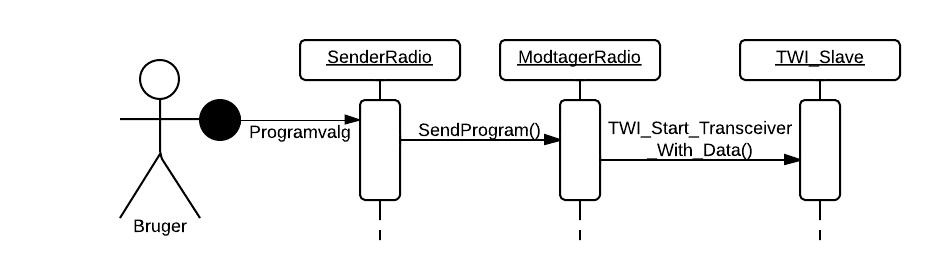
\includegraphics[width = 0.7 \textwidth]{SendProgram}
\caption{Sekvensdiagram fra fjernbetjening til drone.}
\label{Fig:sendProgram}
\end{figure}

\subsubsection*{Deployment View}
Da først der var noget funktionelt på hver enhed, blev kommunikationen imellem enhederne sat op.
Mellem fjernbetjeningen og modtageren skulle der være en 433 MHz forbindelse, som ville styre\dots\fxnote{RBK -- ace dette}


\subsubsection*{Process View}
Koden til dronen, radiosenderen og radiomodtageren er skrevet i programmeringssproget C.

Der er tre projekter at arbejde videre på, beskrevet i næste afsnit.

\subsubsection*{Implementation View}
\begin{itemize}
\item Sender
\item Modtager
\item Drone
\end{itemize}

Det er muligt at videreudvikle på projektet.
En udførlig guide til hvordan man kommer i gang med det, er at finde i  designdokumentet\cite[afs. 2.4]{Design}.















\end{document}
